\chapter{Introducción}
\label{cap:capitulo1}
\setcounter{page}{1}

\begin{flushright}
\begin{minipage}[]{10cm}
\emph{La motivación nos impulsa a comenzar y el hábito nos permite continuar}\\
\end{minipage}\\

Jim Ryun\\
\end{flushright}

\vspace{1cm}

La robótica ha sufrido una transformación enorme a lo largo de su historia aunque siempre teniendo en mente el mismo objetivo: cumplir con el deseo humano. Debido a esa transformación y ese deseo, se ha podido consolidar este campo en la actualidad que abarca cada sector que se pueda imaginar. Otra vertiente que ha destacado en la robótica estos últimos años ha sido la creación de robots de bajo coste para que puedan llegar a un mayor número de personas y se puedan beneficiar de esta ciencia. 

En el presente capítulo se va a abordar el contexto de la robótica, explicando brevemente su historia para poder entender realmente qué es la robótica y lo que es un robot. También se van a encuadrar los tipos de robots que existen y sus múltiples aplicaciones. Todo esto nos ayudará a poder entender mejor dónde se encuadra el presente trabajo, proporcionando los conocimientos necesarios, tanto teóricos como prácticos, que se describirán a lo largo del documento.\\

\section{La robótica}
\label{sec:robotica} % etiqueta para luego referenciar esta sección

La robótica es el campo de la ingeniería que se enfoca en el diseño, la construcción y la programación de robots para tareas específicas. Por ende, un robot se podría definir como un sistema informático formado por sensores y actuadores imprecisos, ya que tienen ruido. Los robots realizan tareas sucias, aburridas y peligrosas y tienen que ser sensibles al entorno. Sin embargo, no existe una definición unívoca al respecto y depende del campo y de la época de la que queramos hablar. Para poder entenderlo, se va a hacer un breve resumen sobre la historia de la robótica.\\

Desde la antigüedad se han desarrollado ingenios o autómatas de los cuáles muchos de ellos tenían fines religiosos como \\


\begin{figure} [h!]
	\begin{center}
		\includegraphics[width=8cm]{figs/memnon}
	\end{center}
	\caption{Colosos de Memnon \cite{memnon_image}}
	\label{fig:memnon}
\end{figure}\

 \textit{incluir imágenes de la estatuas de Memnon \cite{memnon_image} y estatua de Anubis}\\
 
Otras invenciones que destacaban por otras aplicaciones fueron: \\

 \textit{incluir imágenes del tornillos de Arquímedes de Siracusa (287-212 a. C), la eolípila de Herón de Alejandría (10-70 d.C), el león mecánico de Leonardo Da Vinci (1452-1519) y el hombre de palo de Juanelo Turriano (1500-1583) }\\

Durante el siglo XX la ciencia dejó de ser una actividad desarrollada en aislamiento y se desarrolló en laboratorios con más gente. El movimiento del positivismo lógico fomentó las investigaciones ya que este movimiento trataba de dar importancia a la ciencia y dejar de lado la filosofía; también, el contexto de las guerras mundiales y de las bombas nucleares influyeron significativamente en este aspecto. Ya se empieza a acuñar la palabra robot a las distintas creaciones que iban surgiendo como pueden ser:

 \textit{incluir imágenes de  Electro y Sparko (1939) de Westinghouse Electric Corporation y de Isaac Asimov y sus leyes de la robótica }\\


e esta época destacan los siguientes robots: 

En 1969 se construye por el SRI Internacional (Stanford Research Institute) un prototipo experimental llamado Shakey que era una unidad independiente de 1.5 metros, equipado con 2 motores, cámara de televisión y una radio conectada a un ordenador, capaz de navegar en entornos cerrados y estructurados de una forma autónoma. Sus objetivos eran aprender del medio y ser capaz de planificar trayectorias de movimiento y las tareas que le asignaron fueron mover y detectar bloques. Sin embargo, cada movimiento podría tardar más de una hora en computarse y aún así, podrían producirse fallos. A Shakey se le conoce como el primer robot móvil. 

 \textit{incluir imagen de Shakey}\\

Otro robot muy conocido es la carreta de Stanford que era capaz de ver y moverse en cualquier ambiente. Con la cámara que disponía, era capaz calcular y trazar distancias. Sin embargo, tardaba 5 horas en recorrer 30 metros. 

https://web.stanford.edu/~learnest/sail/oldcart.html

 \textit{incluir imagen de carreta Standford}\\
 
Ya a partir de la década de los 80, se decidió que el acceso a los robots fuese para todo el mundo. Lo que provocó asombro, inquietud y miedo ya que el desconocimiento de aquella situación generó rechazo; cosa que ocurre hoy en día. El mundo de la literatura y cine tampoco ayudaba en ese aspecto ya que se presentaba al robot como algo perjudicial para la humanidad. Afortunadamente, esta situación va menguando con el tiempo y se está consiguiendo ver a los robots como un asistente del ser humano que lo que quiere es mejorar su calidad de vida. Para conocer en qué ánbitos un robot puede ayudar al ser humano, es necesario conocer cómo se clasifican. \\


\subsection{Robots industriales}




\subsection{Robots de servicio}



En los textos puedes poner palabras en \textit{cursiva}, para aquellas expresiones en sentido \textit{figurado}, palabras como \textit{robota}, que está fuera del diccionario castellano, o bien para resaltar palabras de una colección: \textit{(a)} es la primera letra del abecedario, \textit{(b)} es la segunda, etc.\\

Al poner las dos líneas del anterior párrafo, este aparecerá separado del anterior. Si no las pongo, los párrafos aparecerán pegados. Sigue el criterio que consideres más oportuno.

\section{Segunda sección}
\label{sec:segundaseccion}

No olvides incluir imágenes y referenciarlas, como la Figura \ref{fig:roomba}.

\begin{figure} [h!]
  \begin{center}
    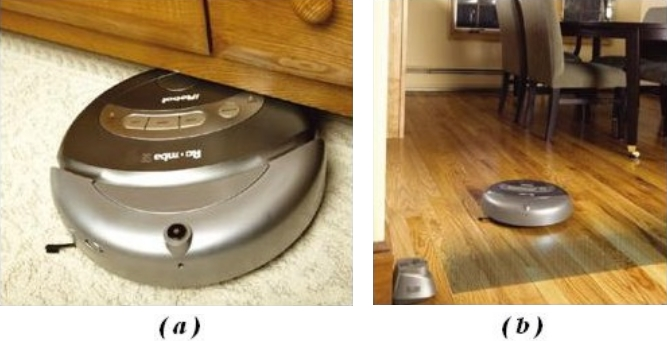
\includegraphics[width=8cm]{figs/roomba}
  \end{center}
  \caption{Robot aspirador Roomba de iRobot.}
  \label{fig:roomba}
\end{figure}\

Ni tampoco olvides de poner las URLs como notas al pie. Por ejemplo, si hablo de la Robocup\footnote{\url{http://www.robocup.org}}.

\subsection{Números}
\label{sec:subseccion}

En lugar de tener secciones interminables, como la Sección \ref{sec:robotica}, divídelas en subsecciones.

Para hablar de números, mételos en el entorno \textit{math} de \LaTeX, por ejemplo, $1.5Kg$. También puedes usar el símbolo del Euro como aquí: 1.500\euro.

\subsection{Listas}

Cuando describas una colección, usa \texttt{itemize} para ítems o \texttt{enumerate} para enumerados. Por ejemplo:

\begin{itemize}
 \item \textit{Entorno de simulación.} Hemos usado dos entornos de simulación: uno en 3D y otro en 2D.
 \item \textit{Entornos reales.} Dentro del campus, hemos realizado experimentos en Biblioteca y en el edificio de Gestión.
\end{itemize}\

\begin{enumerate}
 \item Primer elemento de la colección.
 \item Segundo elemento de la colección.
\end{enumerate}\

\paragraph{Referencias bibliográficas}
\label{sec:referencias}

Cita, sobre todo en este capítulo, referencias bibliográficas que respalden tu argumento. Para citarlas basta con poner la instrucción \verb|\cite| con el identificador de la cita. Por ejemplo: libros como \cite{vega12e}, artículos como \cite{vega19b}, URLs como \cite{vega19a}, tesis como \cite{vega18b}, congresos como \cite{vega18a}, u otros trabajos fin de grado como \cite{vega08b}.

Las referencias, con todo su contenido, están recogidas en el fichero \texttt{bibliografia.bib}. El contenido de estas referencias está en formato \texttt{BibTex}. Este formato se puede obtener en muchas ocasiones directamente, desde plataformas como \texttt{Google Scholar} u otros repositorios de recursos científicos.

Existen numerosos estilos para reflejar una referencia bibliográfica. El estilo establecido por defecto en este documento es APA, que es uno de los estilos más comunes, pero lo puedes modificar en el archivo \texttt{memoria.tex}; concretamente, cambiando el campo \verb|apalike| a otro en la instrucción \verb|\bibliographystyle{apalike}|. 

\

\

\

Y, para terminar este capítulo, resume brevemente qué vas a contar en los siguientes.
